
\documentclass[a4paper,11pt]{article}
\usepackage{verbatim} 
\usepackage{graphicx}
\usepackage{hyperref }
\usepackage[acronym]{glossaries}
%\usepackage[xindy,toc]{glossaries}
\makeglossaries

\title{PyGMO Visualization Manual}
\author{
      Edgar Sim\'{o} Serra \\
      Mentored by Chit-Hong Yam and Dario Izzo 
}
\date{\today}

\begin{document}
\maketitle

\begin{abstract}
Manual for the Visualization module from PyGMO developed for PaGMO as part of the Google Summer of Code 2010 project.
\end{abstract}



\newacronym{API}{API}{Application Programmable Interface}
\newacronym{PaGMO}{PaGMO}{Parallel Global Multiobjective Optimizer}
\newglossaryentry{PyGMO}
{
   name={PyGMO},
   description={Python bindings for PaGMO}
}
\newacronym{GSoC}{GSoC}{Google Summer of Code}
\newglossaryentry{python}
{
   name={Python},
   description={Interpreted, object-oriented, high-level programming language with dynamic semantics}
}
\newglossaryentry{opengl}
{
   name={OpenGL},
   description={Standard specification defining a cross-language, cross-platform API for writing applications that produce 2D and 3D computer graphics}
}
\newacronym{csv}{CSV}{Comma Separated Value}
\newacronym{MGA}{MGA}{Multiple Gravity Assist}
\newacronym{DSM}{DSM}{Deep Space Maneuver}
\newacronym{SI}{SI}{International System of Units}
\newacronym{mjd2000}{MJD2000}{Modified Julian Date 2000}


% The glossary
\printglossaries


\tableofcontents
\newpage

\section{Introduction}
This is the manual for the Visualization module which is part of the \gls{PyGMO} python suite for interaction with \gls{PaGMO}. The objective of this module is 3D Visualization of Interplanetary Trajectories. This manual is intended both for python developers using the PyGMO \gls{API} and end users executing the python script.



\subsection{Requirements}

The main requirement for the visualization module is \gls{python} and \gls{opengl}. Besides this the requirements are very loose. The following should give an approximate idea of what kind of computer is needed to run the visualization module:

\begin{itemize}
\item Pentium II class processor or better
\item 10 MB free dis space
\item 50 MB free RAM
\item OpenGL 1.1 capable card with VBO extension
\end{itemize}

To be able to run the visualization module you must have all the dependencies. The dependency list is:

\begin{itemize}
\item \gls{python}
\item PyOpengl module
\item numpy module
\item PyFTGL module
\item RE module
\item CSV module
\item dateutil module
\end{itemize}


\subsection{Features}

The Visualization module is designed around flexibility and simplicity. 

\paragraph{Feature list:}
\begin{itemize}
\item Visualization of trajectories
\item Ability to add planets
\item Time slider to be able to move to any time instant in the path
\item Keyboard interaction
\item Mouse Interaction that behaves like most 3D applications
\item Support for processing \gls{CSV} files.
\end{itemize}


\section{Installing the Visualization Module}

The installation is not different from the standard \gls{PaGMO} and \gls{PyGMO} installation\cite{install:pagmo}. However care must be taken so that \gls{PyGMO} is also installed.


\section{Using the Visualization Module}

The visualization module has two important aspects. The first is the acquiring of the data and setting up of the window. The second is the moving and manipulating of the trajectory with the window.


\subsection{Python API}

The \gls{python} \gls{API} is aimed at developers although it is simple enough to be used by anyone.

\subsubsection{Getting Started}

To get started with the python


\section{GUI Mock-up}

\begin{comment}
\begin{figure}[ht]
\centering
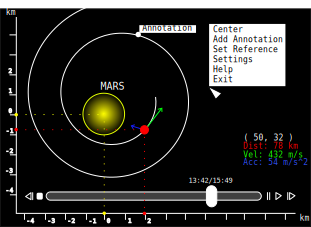
\includegraphics[width=1\textwidth]{mockup}
\caption{Mock-up of the Interface}
\label{fig:mockup}
\end{figure}
\end{comment}

The design of the GUI (Graphical User Interface) is minimalistic. It is meant to be able to fulfil all the required features mentioned before in a comfortable and simple way. By avoiding unneeded options and features, the window is much cleaner and the interface much more simple. This allows it to be comfortable for users of all levels.

In figure \ref{fig:mockup} you can see all the features. There are rulers indicating position relative to the current reference (in this case the reference is Mars). The current position and the current reference are both marked on the rules to make it easier to see. The trajectory is clearly visible for past and future positions and the acceleration and velocity vectors are drawn on the current position. On the bottom there is the time slider, which allows the user to play the entire animation or jump to a specific point in time. It fades out when not being used until the mouse is over it again.

On the right there is both the current position (relative to reference). Below it is the distance from the reference, the current velocity and the current acceleration in numerical values. These can be hidden or be changed to use other units by the settings tab in the menu. To open the menu you just have to right click as shown in figure \ref{fig:mockup}. As you can see there's few items to try to keep the interface simple. The most important being the ability to add annotations, change references and change settings. You can see an annotation on the trajectory in the figure also.

The mock-up is just for reference. The final application will most likely not look like the mock-up but will look similar. 


\section{Interface}

The human interface will consist of two parts. First the user will be able to pass command line arguments to the application, allowing him to configure core settings which can also be saved in a configuration file. This allows scripted settings to be done.

The second and more important interface is the active interface when a trajectory is being visualized. This interface consists of interpreting user input that can come from the mouse or the keyboard to manipulate the visualization. The interface is to be simple and intuitive. This means it should follow the movements of other CAD applications. The more intuitive the interface is, the smaller the learning curve will be for the users. To make the application even more intuitive it should use the context for each input. For example double clicking an object could set it as a reference.

Some of the common mouse functionality is:
\begin{itemize}
\item Rotation with the middle mouse button
\item Zooming with mouse scrolling
\item Shift and drag moves around the plane perpendicular to the camera
\item Clicking selects object
\item Right clicking opens context sensitive menu
\item Double clicking does context sensitive action
\end{itemize}

Some of the common keyboard functionality is:
\begin{itemize}
\item Numpad to move the camera around
\item Hotkeys to different actions to avoid mouse usage for power users
\end{itemize}

The trajectory visualizer will follow the common functionality to simplify the experience for new users.


\section{Conclusions}

There is much more to application design than expected when it comes to ergonomics and intuitiveness. These aspects are often overlooked and can bring problems when the application is finished and no one is able to use it well. By thinking about these aspects before the start of a project, one can already predict where conflicts are most likely to occur and how to avoid them. This is one of the best ways to ensure the quality of the final product like in this case the 3D Visualization for Interplanetary Trajectories.

\bibliographystyle{plain}
\bibliography{manbib}

\end{document}

